\documentclass[a4j]{ujarticle}

\usepackage[dvipdfmx]{graphicx}
\usepackage{graphicx}
\usepackage{url}
\usepackage{listings}
\usepackage{ascmac}
\usepackage{amsmath,amssymb}

\lstset{
  basicstyle={\ttfamily},
  identifierstyle={\small},
  commentstyle={\small\itshape},
  keywordstyle={\small\bfseries},
  ndkeywordstyle={\small},
  stringstyle={\small\ttfamily},
  frame={tb},
  breaklines=true,
  columns=[l]{fullflexible},
  numbers=left,
  xrightmargin=0zw,
  xleftmargin=3zw,
  numberstyle={\scriptsize},
  stepnumber=1,
  numbersep=1zw,
  lineskip=-0.5ex
}

\title{タイトル}
\date{\today}
\author{\input{./authors.txt}}
\begin{document}
\maketitle
\section{概要}
本プロジェクトは、日本語の5文字単語を用いたWordle風パズルゲームである。ユーザーは制限回数内で正解の単語を推測し当てることを目指す。視覚的および操作的な体験(UI/UX)は、本家Wordle(\url{https://wordle.mottox2.com})に準拠している。また、ゲーム開始・履歴表示・終了といった簡易メニュー画面の実装も行った。
\section{プロジェクトの進め方}
本プロジェクトを開始するにあたり、まずは要件定義を行い、必要な機能と非機能要件を明確にした。その後、各自の担当部分を決めて実装を進めた。
\subsection{要件}
\subsubsection{機能要件}
\begin{itemize}
  \item プレイごとにデータベースからランダムで1語を選出
  \item ユーザーによる5文字入力受付
  \item 入力語と正解語の一致度判定
  \begin{itemize}
    \item 正しい文字かつ正しい位置:緑
    \item 正しい文字だが位置が違う:黄
    \item 含まれていない文字:灰
  \end{itemize}
  \item 最大6回まで入力可能(失敗時はGame Over)
  \item 勝敗結果と履歴はデータベースに記録
\end{itemize}

\subsubsection{追加機能(任意)}
\begin{itemize}
  \item メニュー画面(新規プレイ、履歴確認、終了)
  \item 履歴表示(過去のゲームデータ)
\end{itemize}

\subsubsection{非機能要件}
\begin{itemize}
  \item データ永続化のためSQLiteを使用
  \item 単体テストしやすい構造(デザインパターン活用)
  \item 日本語入力対応(IME)
\end{itemize}
\subsection{役割分担}
\begin{description}
  \item[\input{./authorNameShort1.txt}:]\texttt{com.programming.advanced.wordle.service}、\texttt{com.programming.advanced.wordle.model}の実装やテスト、一部の\texttt{GameController}の実装を担当。
  \item[\input{./authorNameShort2.txt}:]\texttt{com.programming.advanced.wordle.dao}におけるDB周りの実装やテスト、DB作成時に利用するリソース(\path{wordle/src/main/resources})の作成を担当。
  \item[\input{./authorNameShort3.txt}:] 
\end{description}
\subsection{開発環境}
本プロジェクトはJavaFXを使用してGUIの構築を行った。エディタにはVSCode、Eclipse、IntelliJ IDEAを使用し、ビルドツールにはMavenを採用した。データベースにはSQLite3を使用し、テストフレームワークにはJUnitを使用した。FXMLファイルの作成には、JavaFX Scene Builderを使用した。\\
バージョン管理システムにはGitを使用し、GitHub上でリポジトリのホスティングを行い共同制作を行った。リポジトリのURLを以下に示す。
\begin{center}
  \url{https://github.com/Punyo/wordle}
\end{center}
また、Discordを用いて定期的に進捗報告や問題の共有を行った。
\section{機能}
\section{実装}
\subsection{DB設計}
本プロジェクトでは、SQLiteを使用してデータの永続化を実現している。データベースには以下の2つのテーブルが存在する。

\begin{figure}[h]
\centering
% 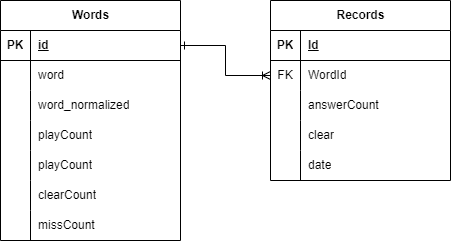
\includegraphics[width=0.8\textwidth]{er.png}
\caption{ER図}
\label{fig:er}
\end{figure}

\subsubsection{Wordsテーブル}
単語データを管理するテーブル。以下のカラムを持つ。
\begin{itemize}
  \item \texttt{id}:単語の一意識別子(INTEGER、PRIMARY KEY、AUTOINCREMENT)
  \item \texttt{word}:単語本体(TEXT、NOT NULL、UNIQUE、CHECK(length(word) = 5))
  \item \texttt{word\_normalized}:正規化された単語(TEXT、NOT NULL、UNIQUE、CHECK(length(word\_normalized) = 5))
  \item \texttt{playCount}:出題された回数(INTEGER、NOT NULL、DEFAULT 0)
  \item \texttt{clearCount}:正解された回数(INTEGER、NOT NULL、DEFAULT 0)
  \item \texttt{missCount}:失敗された回数(INTEGER、NOT NULL、DEFAULT 0)
\end{itemize}

\subsubsection{Recordsテーブル}
プレイ記録を管理するテーブル。以下のカラムを持つ。
\begin{itemize}
  \item \texttt{id}:記録の一意識別子(INTEGER、PRIMARY KEY、AUTOINCREMENT)
  \item \texttt{wordId}:出題された単語のID(INTEGER、NOT NULL、FOREIGN KEY)
  \item \texttt{answerCount}:回答回数(INTEGER、NOT NULL)
  \item \texttt{clear}:正解したかどうか(BOOLEAN、NOT NULL)
  \item \texttt{date}:プレイ日時(DATE、NOT NULL)
\end{itemize}

\subsubsection{インデックス}
検索の効率化のために、以下のインデックスを作成している。
\begin{itemize}
  \item \texttt{idx\_word\_normalized}:Wordsテーブルの\texttt{word\_normalized}カラムに対するインデックス
\end{itemize}

\subsubsection{制約}
データの整合性を保つために、以下の制約を設定している。
\begin{itemize}
  \item Wordsテーブル
  \begin{itemize}
    \item 単語は必ず5文字であること
    \item 単語と正規化された単語は一意であること
  \end{itemize}
  \item Recordsテーブル
  \begin{itemize}
    \item \texttt{wordId}はWordsテーブルの\texttt{id}を参照すること
  \end{itemize}
\end{itemize}

\subsection{com.programming.advanced.wordle.service}
このパッケージには主にゲームの進行管理や判定ロジック等が実装されている。以下のクラスが含まれる。
\begin{itemize}
  \item \texttt{GameService}:ゲームの状態(正解単語、残り試行回数、単語長など)を管理し、ゲームの開始や入力単語の判定処理を行うSingletonであるクラスである。
  \item \texttt{WordBoxStatus}:\texttt{GameService.checkWord(String inputWord)}での判定結果を表す列挙型。
  \item \texttt{GameServiceTest}:\texttt{GameService}のテストクラスで、JUnitを使用してゲームのロジックが正しく動作するかを確認する。
  \item \texttt{GameServiceNotInitializedTest}:\texttt{GameService}が初期化されていない状態でのテストクラスで、ゲームの初期化が行われていない場合の挙動を確認する。
\end{itemize}

それぞれのクラスの詳細を以下に示す。なお、getter/setterは省略する。
\subsubsection{GameService.java}

\begin{itemize}
  \item \texttt{getInstance()}:\texttt{GameService}のインスタンスを取得する。
  \item \texttt{startNewGame(String word, int attempts, int wordLength)}:新しいゲームを開始し、正解単語・試行回数・単語長をセットし、初期化フラグを立てる。
  \item \texttt{checkWord(String inputWord)}:入力単語を正解単語と比較し、各文字ごとに\texttt{WordBoxStatus}(正解・含まれる・含まれない)を判定して返す。試行回数も減少する。\\
  なお、引数の単語が正解の単語の長さと異なる場合、DBからのデータの読み取りに失敗した場合、試行回数が残っていない場合、\texttt{startNewGame} での初期化が行われていなかった場合は例外を投げる。さらに、入力語がDBに登録されていない場合はnullを返す。
\end{itemize}

\subsubsection{WordBoxStatus.java}

\begin{itemize}
  \item \texttt{CORRECT}:文字が正しい位置にある場合。
  \item \texttt{NOT\_IN\_WORD}:文字が単語に含まれない場合。
  \item \texttt{IN\_WORD}:文字が単語に含まれるが位置が違う場合。
\end{itemize}

\subsubsection{GameServiceTest.java}

\begin{itemize}
  \item \texttt{testCheckWordLength()}:入力単語の長さが正解単語と異なる場合に\texttt{IllegalArgumentException}が投げられることを確認するテスト。
  \item \texttt{testCheckWordCorrect()}:正解単語を入力した場合、すべての判定が\texttt{CORRECT}となることを確認するテスト。
  \item \texttt{testCheckWordStatus()}:一部の文字が正解、一部が不正解の場合の判定結果(\texttt{CORRECT}、\texttt{NOT\_IN\_WORD}、\texttt{IN\_WORD})が正しいことを確認するテスト。
  \item \texttt{testCheckWordNoRemainingAttempts()}:試行回数が0になった後に入力した場合、\texttt{IllegalStateException}が投げられることを確認するテスト。
  \item \texttt{testGetters()}:\texttt{GameService}のgetterメソッドが正しく値を返すことを確認するテスト。
\end{itemize}

\subsubsection{GameServiceNotInitializedTest.java}

\begin{itemize}
  \item \texttt{testCheckWordNotInitialized()}:\texttt{GameService}が初期化されていない状態で\texttt{checkWord}を呼び出した場合、\texttt{IllegalStateException}が投げられることを確認するテスト。
\end{itemize}

\subsection{com.programming.advanced.wordle.controller}
このパッケージには、ゲームの各画面を管理するコントローラクラスと、それに関連する機能が実装されている。以下のクラスが含まれる。

\subsubsection{GameController.java}
プレイ画面を管理するコントローラクラス。\texttt{BaseController.java}を継承し、ゲームの進行やユーザー入力の処理を行う。

\begin{itemize}
  \item \texttt{initialize()}:ゲームを初期化し、新しい単語を取得してグリッドとキーボードを構築する。
  \item \texttt{getCurrentRow()}:現在の試行行番号を取得する。
  \item \texttt{getCurrentCell()}:現在の文字入力位置に対応するセルを取得する。
  \item \texttt{setFocusOnCurrentCell()}:現在の入力セルにフォーカスを当てる。
  \item \texttt{putLetterOnCurrentCell(char letter)}:指定した文字を現在のセルに入力し、現在の単語に追加する。
  \item \texttt{setupWordGrid()}:ゲーム用のマス目(TextField)のグリッドを構築し、初期状態の入力可能セルを設定する。
  \item \texttt{createGridCell()}:文字マス(TextField)を生成し、入力された文字をひらがなに変換する処理やフォーカス制御を行う。
  \item \texttt{setupKeyboard()}:50音配列に従って仮想キーボードを構築する。また、BackspaceキーとEnterキーを追加する。
  \item \texttt{createActionKeyButton(String text)}:BackspaceやEnterなどのアクションキーを生成する。
  \item \texttt{handleEnter()}:現在の単語を\texttt{GameService}に渡して判定し、正解またはゲームオーバーならダイアログを表示する。そうでない場合は結果に応じてセルとキーボードの色を更新する。
  \item \texttt{createKeyboardButton(String text)}:文字キーのボタンを生成し、押下時に文字を入力するように設定する。
  \item \texttt{handleBackspace()}:入力中の単語から最後の文字を削除し、対応するセルの表示も削除する。
  \item \texttt{updateCurrentRowCellsColor(WordBoxStatus[] status, int row)}:指定行のセルに判定結果に応じた色を適用する。
  \item \texttt{updateKeyboardColor(WordBoxStatus[] status)}:現在の単語の各文字に対応するキーボードボタンの色を判定結果に基づいて更新する。
  \item \texttt{handleKeyPress(String letter)}:仮想キーボードからの文字入力に応じてセルに文字を入力する。
  \item \texttt{showGameDialog(boolean isClear)}:ゲームクリアまたは失敗時に結果ダイアログを表示し、記録を保存する。
\end{itemize}

\subsubsection{MenuController.java}
メニュー画面を管理するコントローラクラス。
\begin{itemize}
\item \texttt{handlePlayAction(ActionEvent e)}:プレイボタンが押されたときに呼び出され、ゲーム画面(\texttt{game})へ遷移する処理を行う。
\item \texttt{handleRecordAction(ActionEvent e)}:記録ボタンが押されたときに呼び出され、記録表示画面(\texttt{record})へ遷移する処理を行う。
\end{itemize}


\subsubsection{RecordController.java}
記録画面を管理するコントローラクラス。

\begin{itemize}
  \item \texttt{playTableView}:記録を表示するためのテーブルビュー。
  \item \texttt{dateColumn}:ゲームを行った日付を表示するカラム。
  \item \texttt{answerColumn}:ゲームの解答語を表示するカラム。
  \item \texttt{tryCountColumn}:解答までにかかった試行回数を表示するカラム。
  \item \texttt{isClearColumn}:ゲームをクリアしたかどうかのフラグを表示するカラム。「クリア」または「失敗」と表示されるようにカスタマイズされている。
  \item \texttt{initialize()}:
  \begin{itemize}
    \item 各カラムに対して、\texttt{PropertyValueFactory} を用いてデータのプロパティを紐づけている。
    \item \texttt{isClearColumn} に対してカスタムセルファクトリを設定し、クリア状態を日本語で表示。
    \item \texttt{RecordDAO} を利用してデータベースから全記録を取得し、\texttt{ObservableList} に変換してテーブルに設定。
    \item テーブルビューは編集不可・フォーカス不要に設定。
    \item 各カラムは並べ替え可能であり、再配置は不可に設定。
    \item テーブルメニューボタンの非表示化、および自動リサイズポリシーの設定。
  \end{itemize}
\end{itemize}

\subsubsection{GameDialogController.java}
ゲーム終了時に表示するダイアログ画面を管理するコントローラクラス。

\begin{itemize}
\item \texttt{initializeDialog(boolean isGameClear, int tryCount)}:ゲーム終了時の結果に応じて、\texttt{resultLabel} に「ゲームクリア」または「ゲームオーバー」と表示し、\texttt{tryCountLabel} に試行回数を表示する。
\item \texttt{handlePlayAgainButton(ActionEvent e)}:\texttt{GameService} の \texttt{resetGame()} を呼び出してゲーム状態を初期化し、現在のウィンドウを閉じてゲーム画面に遷移する。
\item \texttt{handleReturnToMenuButton(ActionEvent e)}:\texttt{GameService} の \texttt{resetGame()} を呼び出してゲーム状態を初期化し、現在のウィンドウを閉じてメニュー画面に遷移する。
\end{itemize}

\subsubsection{BaseController.java}
\texttt{GameController}と\texttt{MenuController}の親クラスであり、共通する機能を実装している。

\begin{itemize}
\item \texttt{handleReturnToMenuButton(ActionEvent e)}:メニュー画面に遷移する。共通の「戻る」ボタンの処理として、他のコントローラーで継承して使用される。
\end{itemize}

\subsection{com.programming.advanced.wordle.dao}
このパッケージには主にデータベースアクセスに関する実装が含まれている。以下のクラスが含まれる。
\begin{itemize}
  \item \texttt{WordDAO}:単語データの取得や検索を行うクラス。
  \item \texttt{RecordDAO}:プレイ記録の保存や統計情報の更新を行うクラス。
  \item \texttt{DatabaseInitializer}:データベースの初期化やテーブル作成を行うクラス。
\end{itemize}

それぞれのクラスの詳細を以下に示す。

\subsubsection{WordDAO.java}
\begin{itemize}
  \item \texttt{getRandomWord()}:データベースからランダムな単語を1つ取得する。
  \item \texttt{getWordById(int id)}:指定されたIDの単語を取得する。
  \item \texttt{getWordIdByWord(String word)}:指定された単語がデータベースに存在するか確認し、存在する場合はそのIDを返す。
\end{itemize}

\subsubsection{RecordDAO.java}
\begin{itemize}
  \item \texttt{saveRecord(RecordDTO dto)}:プレイ記録を保存し、単語の統計情報(プレイ回数、クリア回数、失敗回数)を更新する。トランザクション管理を行い、データの整合性を保証する。
\end{itemize}

\subsubsection{DatabaseInitializer.java}
\begin{itemize}
  \item \texttt{initializeDatabase()}:データベースの初期化を行う。SQLite JDBCドライバの登録、テーブルの作成、インデックスの作成を行う。
  \item \texttt{insertInitialWords(Connection conn)}:初期データとしてwords.txtから単語を読み込み、データベースに追加する。
\end{itemize}

\subsubsection{DatabaseTest.java}
\begin{itemize}
  \item \texttt{testDatabaseConnection()}:データベースの接続とテーブル構造を確認するテスト。以下の項目を検証する。
  \begin{itemize}
    \item 必要なテーブル(words、records)が存在すること
    \item 各テーブルのカラム定義が正しいこと
  \end{itemize}
  \item \texttt{testSaveRecordAndGetAllRecords()}:レコードの保存と取得をテストする。以下の項目を検証する。
  \begin{itemize}
    \item クリア記録の保存が成功すること
    \item 失敗記録の保存が成功すること
    \item 全レコードの取得が正しく行われること
    \item 最新のレコードが失敗記録であること
    \item 2番目のレコードがクリア記録であること
  \end{itemize}
  \item \texttt{testWordStatisticsUpdate()}:単語の統計情報の更新をテストする。以下の項目を検証する。
  \begin{itemize}
    \item クリア記録保存後の統計情報が正しく更新されること
    \item 失敗記録保存後の統計情報が正しく更新されること
    \item プレイ回数、クリア回数、失敗回数が期待通りに増加すること
  \end{itemize}
\end{itemize}

\subsection{単語データの作成}
\subsubsection{単語データの作成プロセス}
Wordsテーブルに挿入する初期データは、以下の手順で作成した。

\begin{enumerate}
  \item 語彙データの取得
  \begin{itemize}
    \item 松下語学学習ラボ(\url{http://www17408ui.sakura.ne.jp/tatsum/database.html})から語彙データを取得
    \item 取得したデータは、単語とその読み方、品詞情報を含むCSVファイル形式
  \end{itemize}
  
  \item 単語の抽出と変換
  \begin{itemize}
    \item 作成したPythonスクリプト(\texttt{extract\_five\_letter\_words.py})を使用
    \item CSVファイルから5文字の単語を抽出
    \item カタカナの読みをひらがなに変換
    \item 正規化処理を適用(小文字を大文字に変換など)
    \item 重複を除去
  \end{itemize}
  
  \item データベースへの登録
  \begin{itemize}
    \item 抽出した単語を\texttt{words.txt}として保存
    \item データベース初期化時に\texttt{words.txt}から単語を読み込み
    \item 現在のデータ数は2,090個
  \end{itemize}
\end{enumerate}

\subsubsection{extract\_five\_letter\_words.py}
このスクリプトは、データベースに登録する5文字の単語を抽出するために使用される。以下の機能を実装している。
\begin{itemize}
  \item \texttt{katakana\_to\_hiragana(katakana\_str)}:カタカナをひらがなに変換する関数。伸ばし棒(ー)はそのまま保持する。
  \item \texttt{normalize\_word(word)}:単語を正規化する関数。小文字を大文字に変換し、以下の変換を行う。
  \begin{itemize}
    \item ぁ→あ、ぃ→い、ぅ→う、ぇ→え、ぉ→お
    \item っ→つ
    \item ゃ→や、ゅ→ゆ、ょ→よ
  \end{itemize}
  \item \texttt{has\_diacritical\_marks(text)}:テキストに濁点・半濁点が含まれているかを判定する関数。
  \item \texttt{extract\_five\_letter\_words(input\_csv, output\_txt)}:CSVファイルから5文字の単語を抽出し、テキストファイルに出力する関数。以下の条件で単語を抽出する。
  \begin{itemize}
    \item 5文字の単語であること
    \item カタカナのみで構成されていること(伸ばし棒は許可)
    \item 品詞が「名詞-普通名詞-一般」であること
    \item 濁点・半濁点を含まないこと
    \item 正規化後に重複しないこと
  \end{itemize}
\end{itemize}


\subsection{GUIの作成}
JavaFXを使用して作成されたFXMLファイルについてプレビュー画像とともに説明する。それぞれのFXMLファイルは、対応するコントローラクラスと連携して画面のレイアウトや動作を定義している。

\subsubsection{game.fxml}

\begin{itemize}
  \item \texttt{returnToMenuButton}:メニュー画面に戻るためのボタン。\\
  クリック時に\texttt{handleReturnToMenuButton}メソッドが呼び出される。
  \item タイトル:画面上部に「WORDLE」というタイトルを表示する\texttt{Label}。
  \item \texttt{wordgrid}:単語入力用のグリッド。中央に配置され、各セル間に5pxの間隔が設定されている。
  \item \texttt{keyboard}:仮想キーボード用のグリッド。中央に配置され、各キー間に2pxの間隔が設定されている。
\end{itemize}

\begin{figure}[h]
\centering
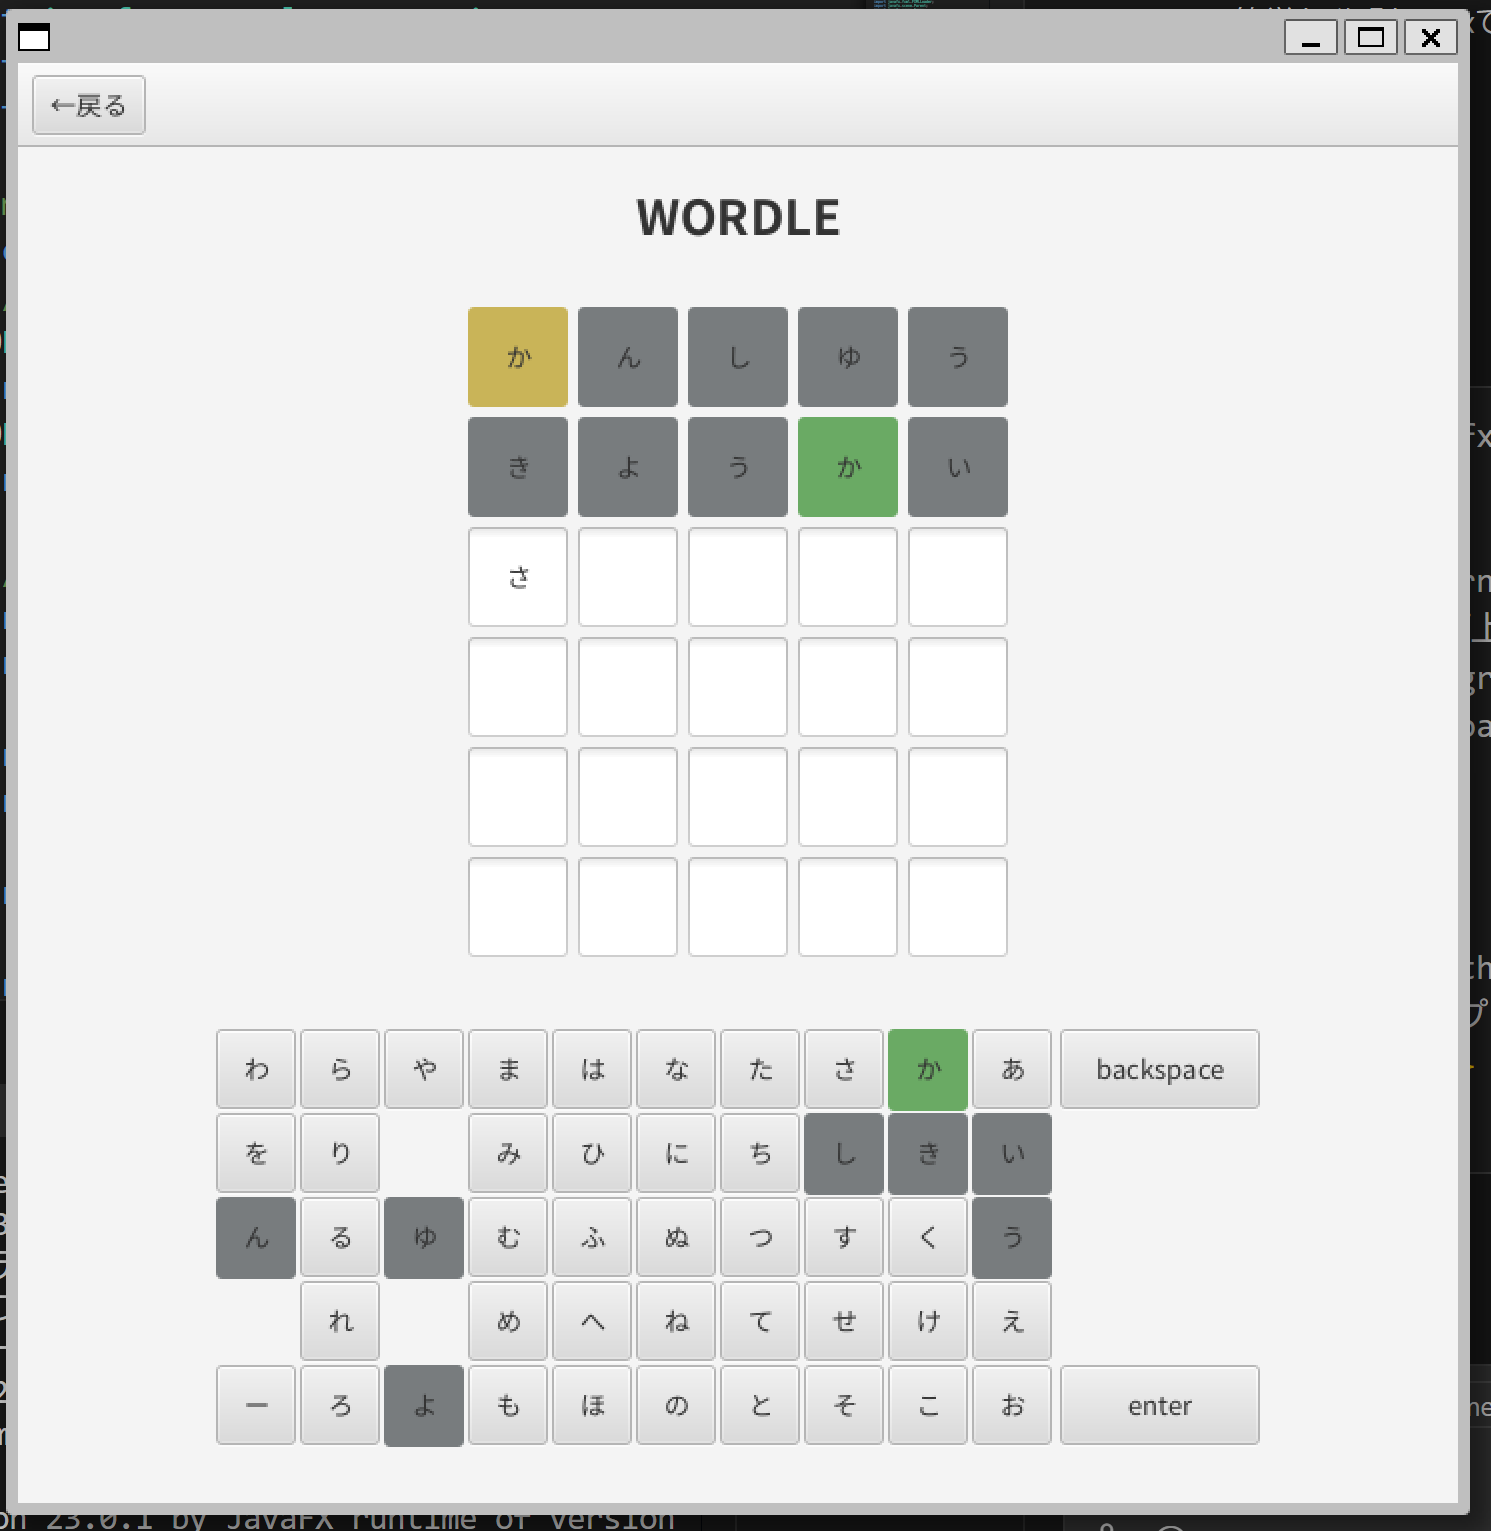
\includegraphics[width=0.8\textwidth]{game_preview.png}
\caption{game.fxmlのプレビュー}
\label{fig:game_fxml}
\end{figure}

\subsubsection{menu.fxml}
\begin{itemize}
  \item タイトル:画面中央上部に「WORDLE」というタイトルを表示する\texttt{Label}。
  \item \texttt{playButton}:ゲームを開始するためのボタン。クリック時に\texttt{handlePlayAction}メソッドが呼び出される。
  \item \texttt{recordButton}:ゲームの記録を確認するためのボタン。クリック時に\texttt{handleRecordAction}メソッドが呼び出される。
\end{itemize}

\begin{figure}[h]
\centering
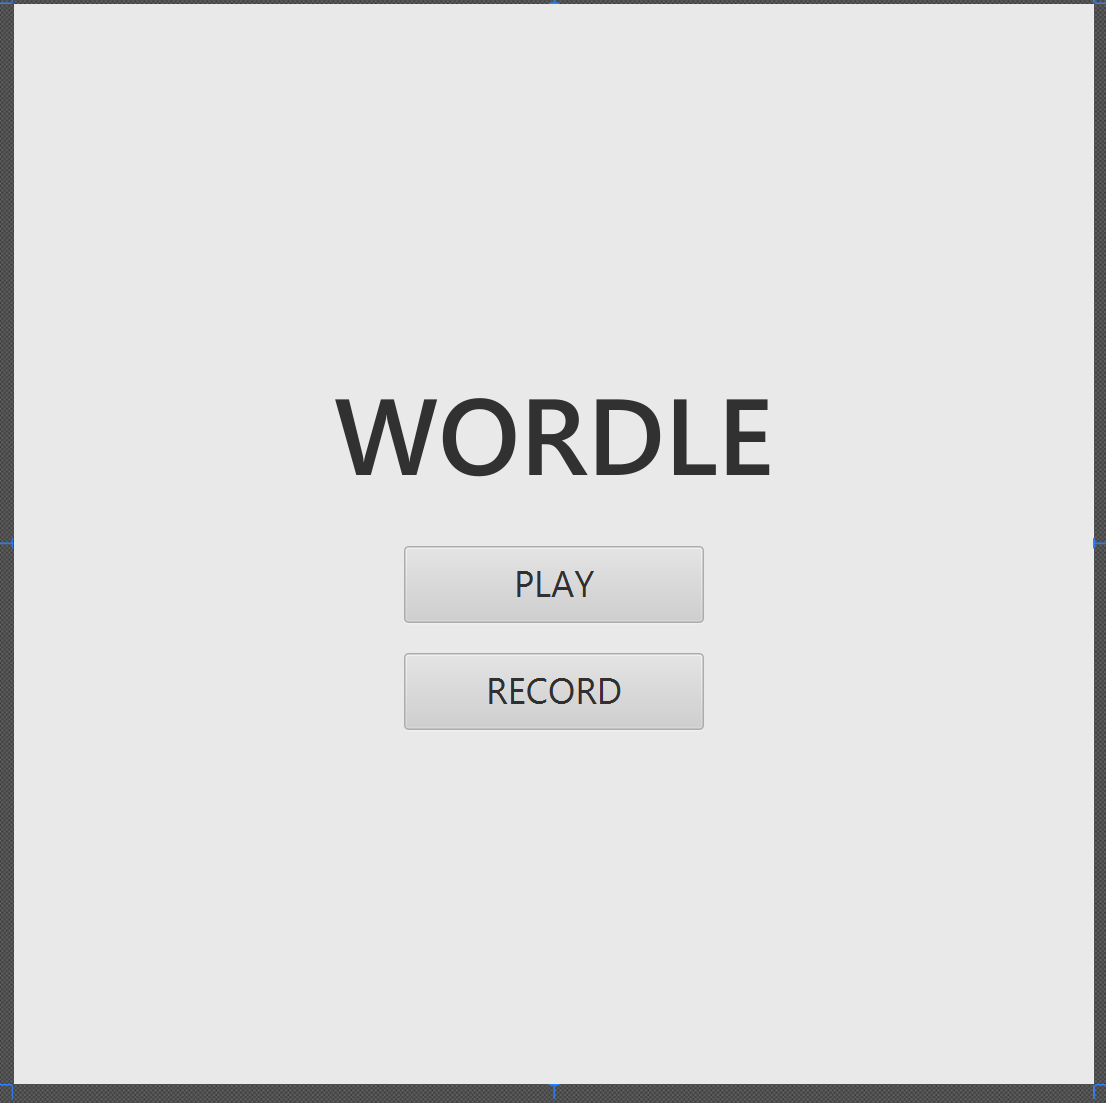
\includegraphics[width=0.8\textwidth]{menu_preview.png}
\caption{menu.fxmlのプレビュー}
\label{fig:menu_fxml}
\end{figure}

\subsubsection{record.fxml}

\begin{itemize}
  \item \texttt{returnToMenuButton}:メニュー画面に戻るためのボタン。クリック時に\texttt{handleReturnToMenuButton}メソッドが呼び出される。
  \item タイトル:画面上部に「遊んだ記録」というタイトルを表示する\texttt{Label}。
  \item \texttt{playTableView}:プレイ記録を表示するテーブルビュー。以下の列を持つ:
  \begin{itemize}
    \item \texttt{dateColumn}:プレイした日付を表示する列。
    \item \texttt{answerColumn}:正解の単語を表示する列。
    \item \texttt{tryCountColumn}:解答回数を表示する列。
    \item \texttt{isClearColumn}:ゲームの結果(クリア/失敗)を表示する列。
  \end{itemize}
\end{itemize}

\begin{figure}[h]
\centering
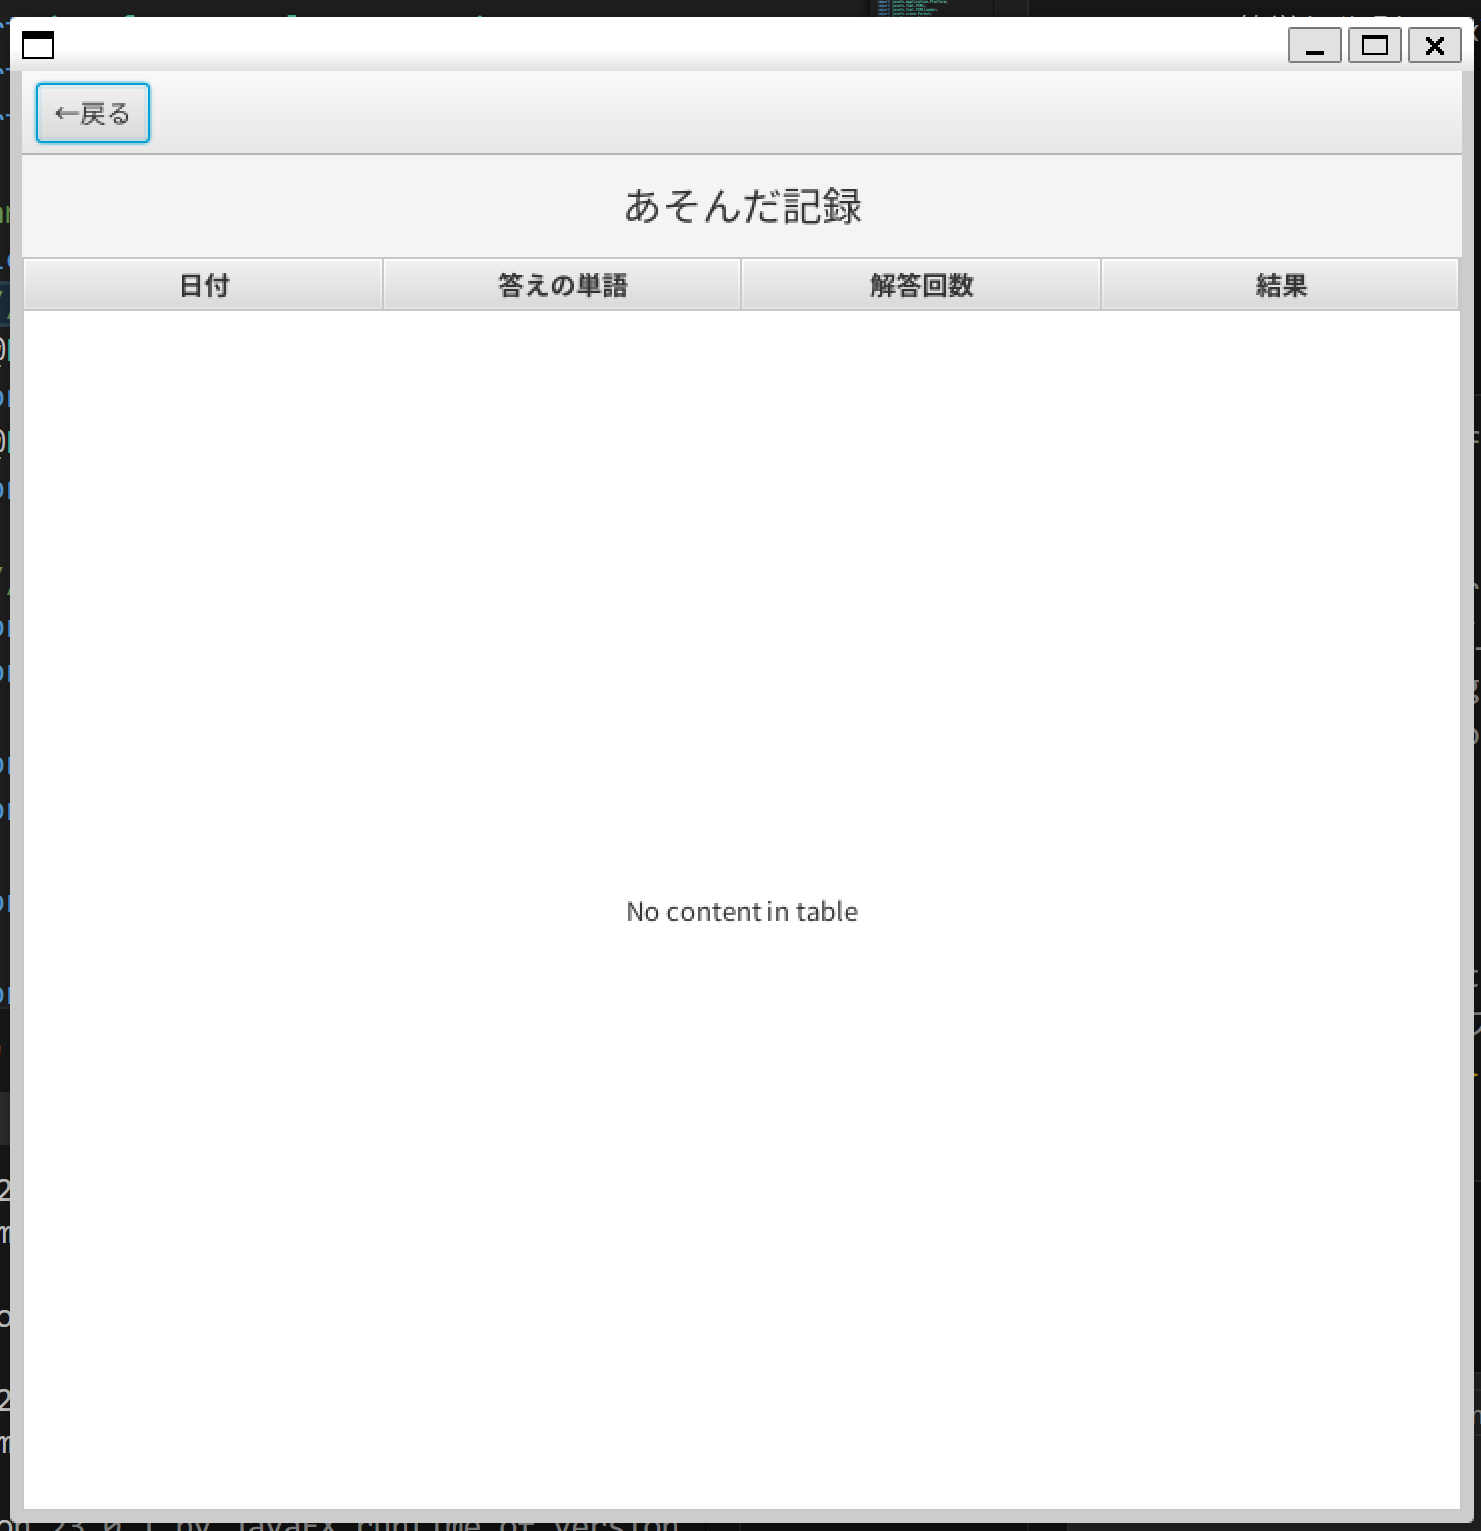
\includegraphics[width=0.8\textwidth]{record_preview.png}
\caption{record.fxmlのプレビュー}
\label{fig:record_fxml}
\end{figure}

\subsubsection{gameDialog.fxml}

\begin{itemize}
  \item \texttt{resultLabel}:ゲームの結果(クリアまたはゲームオーバー)を表示するラベル。
  \item \texttt{answerLabel}:正解の単語を表示するラベル。
  \item \texttt{tryCountLabel}:試行回数を表示するラベル。
  \item \texttt{playAgainButton}:「もう一度プレイする」ボタン。クリック時に\texttt{handlePlayAgainButton}メソッドが呼び出される。
  \item \texttt{returnToMenuButton}:「メニューに戻る」ボタン。クリック時に\texttt{handleReturnToMenuButton}メソッドが呼び出される。
\end{itemize}

\begin{figure}[h]
\centering
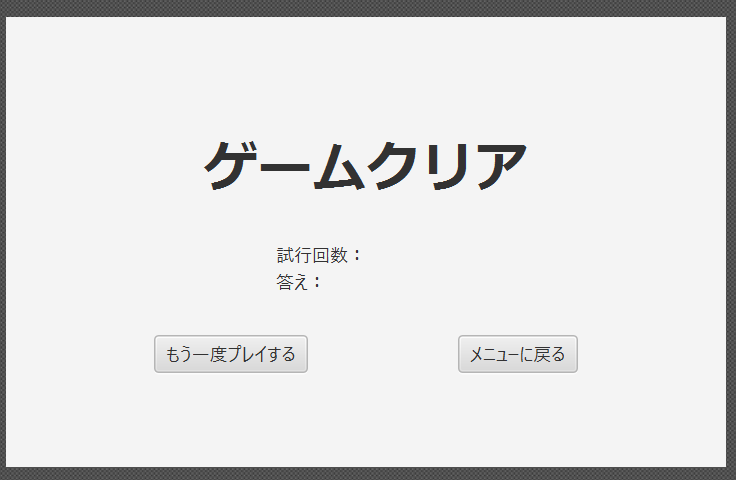
\includegraphics[width=0.8\textwidth]{gameDialog_preview.png}
\caption{gameDialog.fxmlのプレビュー}
\label{fig:gameDialog_fxml}
\end{figure}

\end{document}